
%%%%% Part 1: Dive right into it!

\begin{frame}{100x Speed-Up?}
 \includegraphics[width=\textwidth]{figures/debunking-100x}
 
 \begin{center} \vspace*{0.5cm} \small Proc.~ISCA 2010 \end{center}
\end{frame}




\begin{frame}[fragile]
\frametitle{GPUs: Disillusion}
 \begin{block}{Computing Architecture Schematic}
  \begin{center}
   \includegraphics[width=0.8\textwidth]{figures/cpu-gpu-detail.pdf}
  \end{center}

 \begin{itemize}
  \item Good for large FLOP-intensive tasks, high memory bandwidth
  \item PCI-Express can be a bottleneck
  \item $\gg 10$-fold speedups (usually) not backed by hardware
 \end{itemize}
 \end{block}

\end{frame}




\begin{frame}{100x Speed-Up?}
 \includegraphics[width=\textwidth]{figures/gflops-sp}
 \begin{center}
  Single Precision Peak GFLOP/sec
 \end{center}
\end{frame}

\begin{frame}{100x Speed-Up?}
 \includegraphics[width=\textwidth]{figures/gflops-dp}
 \begin{center}
  Double Precision Peak GFLOP/sec
 \end{center}
\end{frame}

\begin{frame}{100x Speed-Up?}
 \includegraphics[width=\textwidth]{figures/tdp}
 \begin{center}
  Thermal Design Power: 2 CPUs vs. 1 GPU for Fair Comparison
 \end{center}
\end{frame}

\begin{frame}{100x Speed-Up?}
 \includegraphics[width=\textwidth]{figures/gflops-per-watt-dp}
 \begin{center}
  GFLOP/sec per Watt
 \end{center}
\end{frame}

\begin{frame}{100x Speed-Up?}
 \includegraphics[width=\textwidth]{figures/mem-bw}
 \begin{center}
  Memory Bandwidth
 \end{center}
\end{frame}


%%%% Which GPU is right for me?
\begin{frame}{Which Accelerator is Right for Me?}
 
  \begin{block}{Available Accelerators (Rough Sketch, Theoretical Peaks)}

   \begin{center}
    \begin{tabular}{|l|c|c|c|c|c|}
     \hline
      Name             & TFLOP/s & RAM (GB) & GB/s & TDP & Price \\
     \hline
     NVIDIA GTX 580    & 3.0/$\sim$0.2 & 1.5-3.0 & 192 & 244 & \$500   \\
     NVIDIA GTX Titan  & 4.5/1.3  & 6.0     & 288 & 250 & \$$\sim$1k \\
     NVIDIA Tesla 2050 & 1.3/0.5  & 3.0-6.0 & 150 & 225 & \$$\sim$2k \\
     NVIDIA K20        & 3.5/1.2  & 5.0     & 200 & 220 & \$$\sim$3k \\
     \hline
     AMD HD 7970       & 3.5/$\sim$0.9 & 3.0-6.0 & 264 & 250 & \$400 \\
     AMD FirePro W9k   & 4.0/1.0  & 6.0     & 264 & 274 & \$$\sim$3k \\
     \hline
     Intel Xeon Phi    & $\sim$2.0/$\sim$1.0 & 8.0 & 320 & 225 & \$$\sim$3k \\
     \hline
     \hline
     Intel Xeon E5-264x  & 0.2/0.1  & $\sim$64 & $\sim$48 & 100 & \$$\sim$1k \\
     \hline
   \end{tabular}
   \end{center}
  \end{block}

  %\visible<2>{
  \begin{block}{PETSc Considerations}
   \begin{itemize}
    \item Single precision performance doesn't matter
    \item Essentially all kernels memory bandwidth limited
    \item Memory access patterns rather irregular
   \end{itemize}
  \end{block}
  %}

\end{frame}






\begin{frame}[fragile]{GPU Programming Frameworks}
 \begin{center}
  \includegraphics[width=\textwidth]{figures/gpu-programming-comparison}
 \end{center}
\end{frame}

\begin{frame}[fragile]{GPU Programming Frameworks}
 \begin{center}
  \includegraphics[width=\textwidth]{figures/gpu-programming-comparison-1}
 \end{center}
\end{frame}

\begin{frame}[fragile]{GPU Programming Frameworks}
 \begin{center}
  \includegraphics[width=\textwidth]{figures/gpu-programming-comparison-1a}
 \end{center}
\end{frame}

\begin{frame}[fragile]{GPU Programming Frameworks}
 \begin{center}
  \includegraphics[width=\textwidth]{figures/gpu-programming-comparison-2}
 \end{center}
\end{frame}


\begin{frame}[fragile]
\frametitle{GPU Programming Frameworks}
 \begin{block}{NVIDIA CUDA}
  \begin{lstlisting}
// GPU kernel:
__global__ void kernel(double *buffer)
{
  int idx = blockIdx.x * blockDim.x + threadIdx.x;
  buffer[idx] = 42.0;
}

// host code:
int main()
{ 
  ...
  cudaMalloc((void**)&buffer,size);
  kernel<<<blocknum, blockdim>>>(buffer);
  ...
}
  \end{lstlisting} 

  \begin{itemize}
   \item {\color{darkgreen}Convenient}: Almost no additional code required
   \item {\color{darkred}Non-Portable}: Vendor-lock
   \item {\color{darkred}Non-Portable}: Relies on \lstinline|nvcc| being available
  \end{itemize}
 \end{block}

\end{frame}



\begin{frame}[fragile]
\frametitle{GPU Programming Frameworks}
 \begin{block}{NVIDIA CUDA Driver API}
  \begin{lstlisting}
// host code:
int main()
{ 
  ...  
  cudaMalloc((void**)&buffer,size);
  void *args[1] = { &buffer };
  cuModuleLoad(&module, module_file);
  cuModuleGetFunction(&function, module, kernel_name);
  cuLaunchKernel(function, 
                 N, 1, 1, // Nx1x1 blocks
                 1, 1, 1, // 1x1x1 threads
                 0, 0, args, 0)
  ...
}
  \end{lstlisting} 

  \begin{itemize}
   \item {\color{darkgreen}Relief}: No dependency on \lstinline|nvcc|
   \item {\color{darkred}Inconvenient}: Pseudo-Assembly PTX code
   \item {\color{darkred}Non-Portable}: PTX updated with each device generation
  \end{itemize}
 \end{block}

\end{frame}

\begin{frame}[fragile]
\frametitle{GPU Programming Frameworks}
 \begin{block}{NVIDIA CUDA Driver API}
  \begin{lstlisting}
// Generated by NVIDIA NVVM Compiler
// Compiler built on Sun Aug 19 23:20:45 2012
// Driver 304.43

.version 3.0
.target sm_13, texmode_independent
.address_size 32

.entry _k0(
 .param .u32 .ptr .global .align 4 _k0_param_0,
 .param .u32 _k0_param_1,
 .param .u32 .ptr .global .align 4 _k0_param_2,
 .param .u32 _k0_param_3,
 .param .u32 .ptr .global .align 4 _k0_param_4,
 .param .u32 _k0_param_5,
 .param .u32 _k0_param_6,
 .param .u32 _k0_param_7,
 .param .u32 .ptr .global .align 4 _k0_param_8,
 .param .u32 _k0_param_9,
 ...
)
  \end{lstlisting} 
 \end{block}

\end{frame}



\begin{frame}[fragile]
\frametitle{GPU Programming Frameworks}
 \begin{block}{OpenACC and Friends}
  \begin{lstlisting}
void func(...) {
  #pragma acc data pcopyin(A[0:size][0:size])
  {
    #pragma acc kernels loop
    for(int i=0; i< size; i++)
      for(int j=0; j < size; j++)
        A[i][j] = 42;
  }
}

int main()
{
  double A[1337][1337];
  func(A);
}
  \end{lstlisting}

  \begin{itemize}
   \item {\color{darkgreen}Convenient}: Simple OpenMP-type pragma annotations
   \item {\color{darkred}Non-Portable}: Compiler support?
   \item {\color{darkred}Non-Portable}: Insufficient control over memory transfers?
  \end{itemize}
 \end{block}

\end{frame}


\begin{frame}[fragile]
\frametitle{GPU Programming Frameworks}
 \begin{block}{OpenCL}
  \begin{lstlisting}
const char *kernel_string =
"__kernel void mykernel(__global double *buffer) {
  buffer[get_global_id(0)] = 42.0;
};";   

int main() {
  ...
  cl_program my_prog = clCreateProgramWithSource(
         my_context,1,&kernel_string,&source_len,&err);
  clBuildProgram(my_prog,0,NULL,NULL,NULL,NULL);
  cl_kernel my_kernel = clCreateKernel(my_prog,
                          "mykernel",&err);
  clSetKernelArg(my_kernel,0,sizeof(cl_mem),&buffer);
  clEnqueueNDRangeKernel(queue,my_kernel,1,NULL,
               &global_size,&local_size,0,NULL,NULL);
} 
  \end{lstlisting} 

  \begin{itemize}
   \item {\color{darkred}Inconvenient}: Low-level boilerplate code required
   \item {\color{darkgreen}Portable}: Broad hardware support (separate SDKs)
   \item {\color{darkred}Bad News}: No more development effort from NVIDIA
  \end{itemize}
 \end{block}

\end{frame}

\begin{frame}[fragile]{GPU Programming Frameworks}
 \begin{center}
  \includegraphics[width=\textwidth]{figures/gpu-programming-comparison-3}
 \end{center}
\end{frame}


\begin{frame}[fragile]{GPU Programming Frameworks}
 \begin{center}
  \includegraphics[width=\textwidth]{figures/gpu-programming-comparison-4}
 \end{center}
\end{frame}

\begin{frame}[fragile]{GPU Programming Frameworks}
 \begin{center}
  \includegraphics[width=\textwidth]{figures/gpu-programming-comparison-5}
 \end{center}
\end{frame}

\begin{frame}[fragile]{GPU Programming Frameworks}
 \begin{center}
  \includegraphics[width=\textwidth]{figures/gpu-programming-comparison-final}
 \end{center}
\end{frame}


\begin{frame}[fragile]
\frametitle{GPUs: Library Aspects}

 \begin{block}{Challenge: Hardware}
  \begin{itemize}
   \item Portable performance
   \item Auto-tuning
   \item Testing requires many different machines
  \end{itemize}
 \end{block}

 \begin{block}{Challenge: Memory}
  \begin{itemize}
   \item Allocation failures?
   \item Multi-GPU?
   \item PCI-Express bottleneck
  \end{itemize}
 \end{block}

 \begin{block}{Challenge: Programming}
  \begin{itemize}
   \item Kernel language?
   \item Which low-level parameters to expose?
  \end{itemize}
 \end{block}

\end{frame}





%%%%% Part 2

\begin{frame}{Part 2}
 \begin{center}
  \textbf{Part 2: Basic Linear Algebra}
 \end{center}
\end{frame}



\begin{frame}{Linear Algebra on GPUs}

 \begin{block}{Consider Something Simple}
  \begin{itemize}
   \item $x \leftarrow y$, $x,y \in \mathbb{R}^N$, distinct
   \item Usually a simple for-loop, memory-bandwidth limited
  \end{itemize}
 \end{block}

 \begin{center}
  \only<1>{ \includegraphics[width=0.8\textwidth]{figures/vec-gpu-scalar-1} }
  \only<2>{ \includegraphics[width=0.8\textwidth]{figures/vec-gpu-scalar-2} }
  \only<3>{ \includegraphics[width=0.8\textwidth]{figures/vec-gpu-scalar-3} }
  \only<4>{ \includegraphics[width=0.8\textwidth]{figures/vec-gpu-scalar-full} }

  \only<5>{ \includegraphics[width=0.8\textwidth]{figures/vec-gpu-vec-1} }
  \only<6>{ \includegraphics[width=0.8\textwidth]{figures/vec-gpu-vec-full} }
  
  \only<7>{ \includegraphics[width=0.8\textwidth]{figures/vec-cpu-vec-1} }
  \only<8>{ \includegraphics[width=0.8\textwidth]{figures/vec-cpu-vec-full} }
 \end{center}

\end{frame}



\begin{frame}{Linear Algebra on GPUs}

 \begin{block}{Consider Something Simple}
  \begin{itemize}
   \item $x \leftarrow y$, $x,y \in \mathbb{R}^N$, distinct
   \item Usually a simple for-loop, memory-bandwidth limited
  \end{itemize}
 \end{block}

 \begin{block}{Parameters}
  \begin{itemize}
   \item Data Types: \lstinline|double|, \lstinline|double2|, etc.
   \item Blocking: Small segments vs. large blocks
   \item Thread sizes: threads per group, number of thread groups
  \end{itemize}
  \vspace*{-0.3cm}
 \end{block}

\end{frame}


\begin{frame}{Linear Algebra on GPUs}

 \begin{block}{OpenCL Benchmarking Baseline}
  \begin{itemize}
   \item \lstinline|double|
   \item small segments
   \item 128 threads per work group
   \item 128 work groups
  \end{itemize}
 \end{block}

 \begin{block}{Results (GB/sec)} 
  \begin{center}
  \begin{tabular}{|l|c|c|c|c|}
   \hline
   Name           & \footnotesize\lstinline|double|, small, 128x128 & \footnotesize Best & \footnotesize \lstinline|double2|, large, 32x240 \\
   \hline
   NVIDIA GTX 285   & 101 & 134 & 134 \\
   NVIDIA GTX 580   & 150 & 166 & 123 \\
   AMD HD 7970      & 161 & 249 & 140 \\
   INTEL E5-2670 x2 &  32 &  79 &  18 \\
   INTEL Xeon Phi   &  32 &  95 &  21  \\
   \hline
  \end{tabular}
  \end{center}
 \end{block}

\end{frame}






\begin{frame}{Vector Addition Benchmarks}
  \begin{center}
   \includegraphics[width=0.95\textwidth]{figures/vector-timings-1}
  \end{center}
\end{frame}

\begin{frame}{Vector Addition Benchmarks}
  \begin{center}
   \includegraphics[width=0.95\textwidth]{figures/vector-timings-2}
  \end{center}
\end{frame}

\begin{frame}{Vector Addition Benchmarks}
  \begin{center}
   \includegraphics[width=0.95\textwidth]{figures/vector-timings-3}
  \end{center}
\end{frame}

\begin{frame}{Vector Addition Benchmarks}
  \begin{center}
   \includegraphics[width=0.95\textwidth]{figures/vector-timings-4}
  \end{center}
\end{frame}

\begin{frame}{Vector Addition Benchmarks}
  \begin{center}
   \includegraphics[width=0.95\textwidth]{figures/vector-timings-5}
  \end{center}
\end{frame}

\begin{frame}{Vector Addition Benchmarks}
  \begin{center}
   \includegraphics[width=0.95\textwidth]{figures/vector-timings-6}
  \end{center}
\end{frame}

\begin{frame}{Vector Addition Benchmarks}
  \begin{center}
   \includegraphics[width=0.95\textwidth]{figures/vector-timings-7}
  \end{center}
\end{frame}



\begin{frame}{Matrix-Matrix Multiplication}
 \begin{block}{Parameter Space Explosion}
  \begin{itemize}
   \item Global Block Sizes
   \item Shared Mem Block Sizes
   \item Thread-Private Block Sizes
   \item Loop Unrolling
  \end{itemize}
 \end{block}
 
   \begin{center}
   \includegraphics[width=0.95\textwidth]{figures/MatrixMatrixProduct}
  \end{center}

\end{frame}



\begin{frame}{Matrix-Matrix Multiplication}
  \begin{center}
   \includegraphics[width=0.95\textwidth]{figures/dgemm}
  \end{center}
\end{frame}

\begin{frame}{Matrix-Matrix Multiplication}
  \begin{center}
   \includegraphics[width=0.95\textwidth]{figures/cross-benchmark-3-double}
  \end{center}
\end{frame}





%%%%% Part 3

\begin{frame}{Part 3}
 \begin{center}
  \textbf{Part 3: Preconditioners}
 \end{center}
\end{frame}




\begin{frame}{Multigrid}

 \begin{minipage}{0.6\textwidth}
 \begin{block}{Ingredients of Algebraic Multigrid}
  \begin{itemize}
   \item Smoother (Relaxation schemes, etc.)
   \item Coarsening
   \item Interpolation (Inter-grid transfer)
  \end{itemize}
 \end{block}
 \end{minipage}

 \begin{minipage}{0.48\textwidth}
  \begin{center}
  \includegraphics[width=0.99\textwidth]{figures/graph-rs.pdf} \\
    Classical coarsening
  \end{center}
 \end{minipage}
 \begin{minipage}{0.48\textwidth}
  \begin{center}
    \includegraphics[width=0.99\textwidth]{figures/graph-ag.pdf} \\
    Aggregation coarsening
  \end{center}
 \end{minipage}
 \vspace*{.5cm}
\end{frame}



%%%%%%%%


\begin{frame}{Multigrid Parallelization}

 \begin{block}{Setup Phase}
  \begin{itemize}
   \item Determination of coarse points in parallel by graph splitting
   \item Compute coarse operators $A^{k+1} = R^k A^k P^k$ (where $A^0 = A$)
   \item Datastructures: analyze and allocate
   \item Limited fine-grained parallelism
  \end{itemize}
 \end{block}

 %\pause
 \begin{minipage}{0.58\textwidth}
 \begin{block}{Cycle Phase}
  \begin{itemize}
   \item Parallel Jacobi Smoother
   \item Restriction $R^k x^k$, prolongation $P^k x^{k+1}$
   \item Direct solution on coarsest level
   \item Static datastructures
   \item Enough fine-grained parallelism
  \end{itemize}
 \end{block}
 \end{minipage}
 \begin{minipage}{0.4\textwidth} \vspace*{-1.5cm}
  \includegraphics[width=0.99\textwidth]{figures/graph-rs0.pdf} \\ \vspace*{0.1cm}
  \includegraphics[width=0.99\textwidth]{figures/multigrid-cycles.png}
 \end{minipage}

 \vspace*{0.5cm}

\end{frame}


%%%%%%%%%%

\begin{frame}{AMG Sparse Matrix-Matrix Multiplication}
 \begin{block}{Coarse Grid Operator}
  \begin{itemize}
   \item $A^{\mathrm{coarse}} = R A^{\mathrm{fine}} P$
   \item Common choice: $R = P^{\mathrm{T}}$
  \end{itemize}
 \end{block}

 \begin{block}{Computation}
  \begin{itemize}
   \item Explicitly set up $R = P^{\mathrm{T}}$ (hard in parallel)
   \item $C = A^{\mathrm{fine}} P$
   \item $A^{\mathrm{coarse}} = R C$
  \end{itemize}
 \end{block}

\end{frame}


\begin{frame}{AMG Sparse Matrix-Matrix Multiplication}
  \begin{center}
    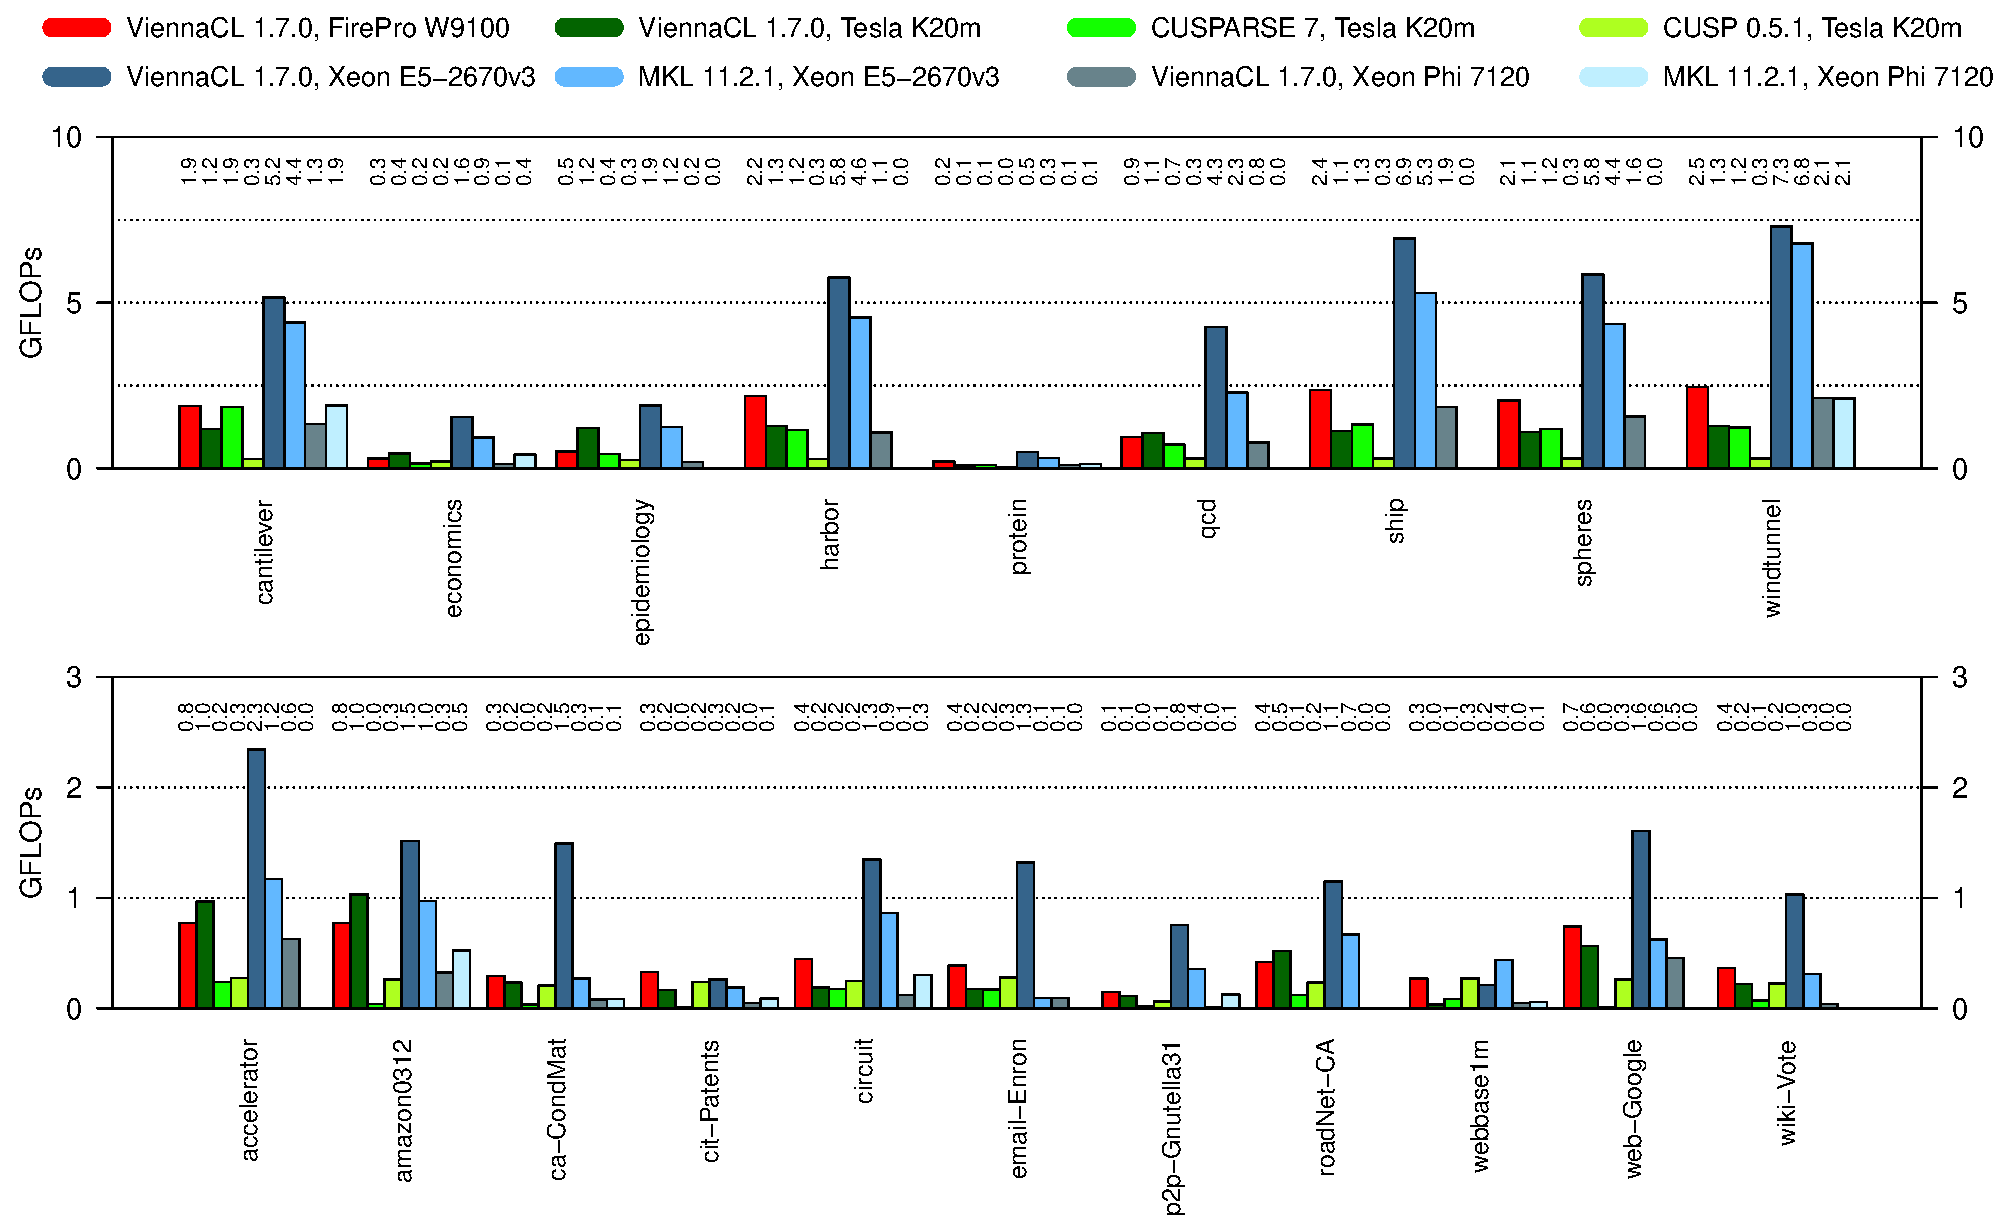
\includegraphics[width=0.95\textwidth]{spgemm}
  \end{center}
\end{frame}


%%%%%%%%%%%%


\begin{frame}{AMG Benchmark}
  \begin{center}
    \includegraphics[width=0.95\textwidth]{amg-vs-pure-full-2d-4}
  \end{center}
\end{frame}




%%
%%%%%%%%%%%% Coloring: Rework ILU example, mention limitations
%%



\begin{frame}[fragile]{Memory Bandwidth vs. Parallelism}
 \begin{center}
  \includegraphics[width=0.95\textwidth]{figures/stream}
 \end{center}
 {\scriptsize https://www.karlrupp.net/2015/02/stream-benchmark-results-on-intel-xeon-and-xeon-phi/ }
\end{frame}



\begin{frame}[fragile]
\frametitle{Parallel ILU}

  \begin{minipage}{0.5\textwidth}
    \begin{block}{ILU - Basic Idea}
      \begin{itemize}
        \item Factor sparse matrix $\matrix A \approx \tilde{\matrix L} \tilde{\matrix U}$
        \item $\tilde{\matrix L}$ and $\tilde{\matrix U}$ sparse, triangular
        \item ILU0: Pattern of $\tilde{\matrix L}$, $\tilde{\matrix U}$ equal to $\matrix A$
        \item ILUT: Keep $k$ elements per row
      \end{itemize}
    \end{block}
  \end{minipage}
%
  \begin{minipage}{0.45\textwidth}
    \begin{block}{Solver Cycle Phase}
      \vspace*{-0.1cm}
      \begin{itemize}
        \item Residual correction ${\color{red}\tilde{\matrix L}} \tilde{\matrix U} x = z$
        \item Forward solve ${\color{red}\tilde{\matrix L}} y = z$
        \item Backward solve $\tilde{\matrix U} x = y$
        \item Little parallelism in general
      \end{itemize}
    \end{block}
  \end{minipage}


  \begin{align*} 
   \left(
   \begin{array}{ccccccccc}
     \textstyle 5 &  \textstyle \times & \textstyle \times     & \textstyle \times  &   & \textstyle \times     & \textstyle \times &   &   \\
     \textstyle \color{red} \times & \textstyle 3 & \textstyle \times      &    &   &      &   &  &   \\
    \textstyle \color{red} \times & \textstyle \color{red} \times & \textstyle 4     & \textstyle \times  &   &       &   &   &   \\
%
    \textstyle \color{red} \times &   &  \textstyle\color{red}  \times     & \textstyle 5  & \textstyle \times & \textstyle \times     &   &   & \textstyle \times \\
      &   &       & \textstyle \color{red} \times  & \textstyle 5 & \textstyle \times     &   & \textstyle \times & \textstyle \times \\
    \textstyle \color{red} \times &   &      & \textstyle \color{red} \times  & \textstyle \color{red} \times & \textstyle 6     & \textstyle \times & \textstyle \times &  \\
%
    \textstyle \color{red} \times &  &       &    &   & \textstyle\color{red}  \times     & \textstyle 3 &   &   \\
      &   &       &    & \textstyle\color{red}  \times & \textstyle \color{red} \times    &   & \textstyle 4 & \textstyle \times \\
      &   &      & \textstyle\color{red}  \times  & \textstyle \color{red} \times &      &   & \textstyle \color{red} \times & \textstyle 4 \\
   \end{array}
         \right)
  \end{align*}

 
\end{frame}





\begin{frame}[fragile]
\frametitle{Parallel ILU}

     \begin{block}{ILU Level Scheduling}
      \begin{itemize}
        \item Build dependency graph
        \item Substitute as many entries as possible simultaneously
        \item Trade-off: Each step vs. multiple steps in a single kernel
      \end{itemize}

      \begin{center}
    \includegraphics[width=0.65\textwidth]{figures/level-scheduling-3.png}
      \end{center}

    \end{block}
\end{frame}


\begin{frame}[fragile]
\frametitle{Parallel ILU}

     \begin{block}{ILU Interpretation on Structured Grids}
      \begin{itemize}
        \item 2d finite-difference discretization
        \item Substitution whenever all neighbors with smaller index computed
        \item Works particularly well in 3d
      \end{itemize}

      \begin{center}
    \only<1>{\includegraphics[width=0.4\textwidth]{figures/2d-grid-1}\hspace*{1.0cm}\includegraphics[width=0.4\textwidth]{figures/order_lexi}}
    \only<2>{\hspace*{-0.085cm}\includegraphics[width=0.4\textwidth]{figures/2d-grid-2}\hspace*{1.0cm}\includegraphics[width=0.4\textwidth]{figures/order_lexi}}
    \only<3>{\hspace*{-0.17cm}\includegraphics[width=0.4\textwidth]{figures/2d-grid-3}\hspace*{1.0cm}\includegraphics[width=0.4\textwidth]{figures/order_lexi}}
%
    \only<4>{\hspace*{-0.255cm}\includegraphics[width=0.4\textwidth]{figures/2d-grid-1-bad}\hspace*{1.0cm}\includegraphics[width=0.4\textwidth]{figures/order_bad}}
    \only<5>{\hspace*{-0.34cm}\includegraphics[width=0.4\textwidth]{figures/2d-grid-2-bad}\hspace*{1.0cm}\includegraphics[width=0.4\textwidth]{figures/order_bad}}
    \only<6>{\hspace*{-0.425cm}\includegraphics[width=0.4\textwidth]{figures/2d-grid-3-bad}\hspace*{1.0cm}\includegraphics[width=0.4\textwidth]{figures/order_bad}}
%
    \only<7>{\hspace*{-0.51cm}\includegraphics[width=0.4\textwidth]{figures/2d-grid-1-min}\hspace*{1.0cm}\includegraphics[width=0.4\textwidth]{figures/order_min}}
    \only<8>{\hspace*{-0.595cm}\includegraphics[width=0.4\textwidth]{figures/2d-grid-2-min}\hspace*{1.0cm}\includegraphics[width=0.4\textwidth]{figures/order_min}}
    \only<9>{\hspace*{-0.68cm}\includegraphics[width=0.4\textwidth]{figures/2d-grid-3-min}\hspace*{1.0cm}\includegraphics[width=0.4\textwidth]{figures/order_min}}
%
    \only<10>{\hspace*{-0.765cm}\includegraphics[width=0.4\textwidth]{figures/2d-grid-1-rb}\hspace*{1.0cm}\includegraphics[width=0.4\textwidth]{figures/order_rb}}
    \only<11>{\hspace*{-0.75cm}\includegraphics[width=0.41\textwidth]{figures/2d-grid-2-rb}\hspace*{0.9cm}\includegraphics[width=0.4\textwidth]{figures/order_rb}}
    \only<12>{\hspace*{-0.75cm}\includegraphics[width=0.41\textwidth]{figures/2d-grid-3-rb}\hspace*{0.9cm}\includegraphics[width=0.4\textwidth]{figures/order_rb}}
      \end{center}

    \end{block}
\end{frame}



\begin{frame}[fragile]{Parallel ILU}

\begin{minipage}{0.45\textwidth}
  Sequential \\
  \lstinline|for i=2..n| \\
  \lstinline|  for k=1..i-1, (i,k) in A| \\
  \hspace*{0.7cm}$a_{ik} =  a_{ik}/a_{kk}$ \\
  \hspace*{0.7cm}\lstinline|for j=k+1..n, (i,j) in A| \\
  \hspace*{1cm}$a_{ij} =  a_{ij} - a_{ik}a_{kj}$ \\
\end{minipage} \hfill
\begin{minipage}{0.5\textwidth}
  Parallel \\
  \lstinline|for (sweep = 1, 2, ...)| \\
  \lstinline|  parallel for (i,j) in A| \\
  \lstinline|    if (i > j)| \\ 
  \hspace*{1cm}$l_{ij} =  (a_{ij} - \sum_{k=1}^{j=1} l_{ik}u_{kj}) / u_{jj}$ \\
  \lstinline|    else| \\
  \hspace*{1cm}$u_{ij} =  a_{ij} - \sum_{k=1}^{=1} l_{ik}u_{kj}$
\end{minipage}


  \begin{block}{Fine-Grained Parallel ILU Setup}
   \begin{itemize}
    \item Proposed by Chow and Patel (SISC, vol.~37(2)) for CPUs and MICs
    \item Massively parallel (one thread per row)
   \end{itemize}
  \end{block}
  
  %\pause
  
  \begin{block}{Preconditioner Application}
   \begin{itemize}
    \item Truncated Neumann series:
     \begin{align*} \mathbf{L}^{-1} \approx \sum_{k=0}^K (\mathbf{I} - \mathbf{L})^k, \quad \mathbf{U}^{-1} \approx \sum_{k=0}^K (\mathbf{I} - \mathbf{U})^k \end{align*}
    \item Exact triangular solves not necessary
   \end{itemize}
  \end{block}

\end{frame}


\begin{frame}{Parallel ILU}
  \begin{center}
    \includegraphics[width=0.95\textwidth]{ilu-2d-4}
  \end{center}
\end{frame}





\begin{frame}[fragile]
\frametitle{Incomplete LU Factorization Preconditioners}

     \begin{block}{Level Scheduling}
      \begin{itemize}
        \item Build dependency graph
        \item Substitute as many entries as possible simultaneously
        \item Trade-off: Each step vs. multiple steps in a single kernel
      \end{itemize}

      \begin{center}
    \only<1>{ \includegraphics[width=0.65\textwidth]{figures/level-scheduling.png} }
    \only<2>{ \includegraphics[width=0.65\textwidth]{figures/level-scheduling-1.png} }
    \only<3>{ \includegraphics[width=0.65\textwidth]{figures/level-scheduling-3.png} }
      \end{center}

    \end{block}
\end{frame}


\begin{frame}[fragile]
\frametitle{Incomplete LU Factorization Preconditioners}

     \begin{block}{Interpretation on Structured Grids}
      \begin{itemize}
        \item 2d finite-difference discretization
        \item Substitution whenever all neighbors with smaller index computed
        \item Works particularly well in 3d
      \end{itemize}

      \begin{center}
    \only<1>{\includegraphics[width=0.4\textwidth]{figures/2d-grid-1}\hspace*{1.0cm}\includegraphics[width=0.4\textwidth]{figures/order_lexi}}
    \only<2>{\hspace*{-0.085cm}\includegraphics[width=0.4\textwidth]{figures/2d-grid-2}\hspace*{1.0cm}\includegraphics[width=0.4\textwidth]{figures/order_lexi}}
    \only<3>{\hspace*{-0.17cm}\includegraphics[width=0.4\textwidth]{figures/2d-grid-3}\hspace*{1.0cm}\includegraphics[width=0.4\textwidth]{figures/order_lexi}}
%
    \only<4>{\hspace*{-0.255cm}\includegraphics[width=0.4\textwidth]{figures/2d-grid-1-bad}\hspace*{1.0cm}\includegraphics[width=0.4\textwidth]{figures/order_bad}}
    \only<5>{\hspace*{-0.34cm}\includegraphics[width=0.4\textwidth]{figures/2d-grid-2-bad}\hspace*{1.0cm}\includegraphics[width=0.4\textwidth]{figures/order_bad}}
    \only<6>{\hspace*{-0.425cm}\includegraphics[width=0.4\textwidth]{figures/2d-grid-3-bad}\hspace*{1.0cm}\includegraphics[width=0.4\textwidth]{figures/order_bad}}
%
    \only<7>{\hspace*{-0.765cm}\includegraphics[width=0.4\textwidth]{figures/2d-grid-1-rb}\hspace*{1.0cm}\includegraphics[width=0.4\textwidth]{figures/order_rb}}
    \only<8>{\hspace*{-0.75cm}\includegraphics[width=0.41\textwidth]{figures/2d-grid-2-rb}\hspace*{0.9cm}\includegraphics[width=0.4\textwidth]{figures/order_rb}}
    \only<9>{\hspace*{-0.75cm}\includegraphics[width=0.41\textwidth]{figures/2d-grid-3-rb}\hspace*{0.9cm}\includegraphics[width=0.4\textwidth]{figures/order_rb}}
      \end{center}

    \end{block}
\end{frame}





\begin{frame}[fragile]
\frametitle{Incomplete LU Factorization Preconditioners}

     \begin{block}{Block-ILU}
      \begin{itemize}
        \item Apply ILU to diagonal blocks
        \item Higher parallelism
        \item Usually more iterations required (problem-dependent)
      \end{itemize}

      \begin{center}
    \only<1>{ \includegraphics[width=0.65\textwidth]{figures/block-ilu.png} }
    \only<2>{ \includegraphics[width=0.65\textwidth]{figures/block-ilu-2.png} }
      \end{center}

    \end{block}


\end{frame}







%%%%%%%%% Benchmarks
\begin{frame}{Benchmark}
 \begin{center}
  Benchmark - Setup
 \end{center}
\end{frame}

\begin{frame}[fragile]
\frametitle{Benchmark Setup}

     \begin{block}{Hardware}
       \begin{itemize}
         \item NVIDIA GTX 580 (default)
         \item AMD HD 7970 (only for final benchmark)
         \item Intel Core2Quad 9550
       \end{itemize}
     \end{block}

     \begin{block}{Numbering}
      \begin{itemize}
        \item Lexicographic
        \item Red-Black
        \item Minimum Degree
      \end{itemize}
    \end{block}

     \begin{block}{Remarks}
      \begin{itemize}
        \item Setup purely on CPU, not included
        \item Data transfer costs not included
        \item OpenCL for both GPUs
      \end{itemize}
    \end{block}

\end{frame}


%%%%%%%%%%% FDM 2D %%%%%%%%%%%%%%%%%%
\begin{frame}{Benchmark}
 \begin{center}
  Case Study 1: 2D Poisson, Structured Grid
 \end{center}
\end{frame}

\begin{frame}{Benchmarks}
  \begin{center}
   \vspace*{-0.4cm}
   \includegraphics[width=0.60\textwidth]{figures/fdm2d-solver.pdf} \\[-0.2em]
   \includegraphics[width=0.60\textwidth]{figures/fdm2d-iters.pdf}
  \end{center}
\end{frame}

\begin{frame}{Benchmarks}
  \begin{center}
   \vspace*{-0.4cm}
   \includegraphics[width=0.60\textwidth]{figures/fdm2d-precond.pdf} \\[-0.2em]
   \includegraphics[width=0.60\textwidth]{figures/fdm2d-levels.pdf}
  \end{center}
\end{frame}


\begin{frame}[fragile]
\frametitle{Incomplete LU Factorization Preconditioners}

     \begin{block}{Coloring}
      \begin{itemize}
        \item Color dependency graph
        \item Purely algebraic
      \end{itemize}

      \begin{center}
    \only<1>{\includegraphics[width=0.65\textwidth]{figures/2d-unstructured-1}}
    \only<2>{\includegraphics[width=0.65\textwidth]{figures/2d-unstructured-2}}
    \only<3>{\includegraphics[width=0.65\textwidth]{figures/2d-unstructured-3}}
      \end{center}

    \end{block}
\end{frame}


\begin{frame}{Benchmarks}
  \begin{center}
   \includegraphics[width=0.90\textwidth]{figures/fem2d-solver-coloring.pdf}
  \end{center}
\end{frame}





%%%% Conclusion


\begin{frame}[fragile]{GPU Programming Conclusion}
 \begin{center}
  \includegraphics[width=\textwidth]{figures/gpu-programming-comparison-final}
 \end{center}
\end{frame}

\begin{frame}[fragile]{GPU Programming Conclusion}
 \begin{center}
  \includegraphics[width=\textwidth]{figures/gpu-programming-comparison-final-libraries}
 \end{center}
\end{frame}
